\documentclass{article}
\usepackage[utf8]{inputenc}
\usepackage[spanish.mexico]{babel}
\usepackage[american voltages, american currents,siunitx]{circuitikz}

%para fotos

\usepackage{graphicx}
\usepackage{subcaption}

\title{Previo 2}
\author{Pablo Vivar Colina\\
Grupo 13\\
}
%\date{Septiembre 2017}

\usepackage{natbib}
\usepackage{graphicx}

\begin{document}

\maketitle

\section{Símbolo}

Un símbolo es la representación perceptible de una idea, con rasgos asociados por una convención socialmente aceptada. Es un signo sin semejanza ni contigüidad, que solamente posee un vínculo convencional entre su significante y su denotado, además de una clase intencional para su designado.\citep{Sim}

\section{Elementos activos y pasivos en un circuito eléctrico}

\subsection{Elementos Pasivos}

Elementos pasivos son aquellos componentes de los circuitos, que disipan o almacenan energía eléctrica o magnética y constituyen por ello los receptores o cargas de un circuito. Estos elementos son modelos matemáticos lineales e ideales de los elementos físicos del circuito.\citep{EAP}\\

pueden presentar las siguientes propiedades:

\begin{enumerate}
    \item disipación de energía eléctrica (R: resistencia)
    \item almacenamiento de energía en campos magnéticos (L: coef. de autoinducción)
    \item almacenamiento de energía en campos eléctricos (C: capacidad).
\end{enumerate}
 
 Como ejemplo se encuentran la resistencia, inductancia y capacitancia.\citep{EAP}\\
 
 \subsection{Elementos Activos}
 
  Los componentes activos son aquellos que son capaces de excitar los circuitos o de realizar ganancias o control del mismo. Fundamentalmente son los generadores eléctricos y ciertos componentes semiconductores.\citep{EAP}\\
  
    Los generadores de corriente mantienen las características de la corriente entre sus bornes, independientemente de los elementos que componen el resto del circuito. Cuando esto no ocurre así se dice que se comporta como un generador real de corriente.\citep{EAP}\\

\section{Osciloscopio}

Un osciloscopio es un instrumento de visualización electrónico para la representación gráfica de señales eléctricas que pueden variar en el tiempo. Es muy usado en electrónica de señal, frecuentemente junto a un analizador de espectro.\citep{Osc}

Presenta los valores de las señales eléctricas en forma de coordenadas en una pantalla, en la que normalmente el eje X (horizontal) representa tiempos y el eje Y (vertical) representa tensiones. La imagen así obtenida se denomina oscilograma.\citep{Osc} 

\section{Las matemáticas y la CA sinusoidal}

Algunos tipos de oscilaciones periódicas tienen el inconveniente de no tener definida su expresión matemática, por lo que no se puede operar analíticamente con ellas. Por el contrario, la oscilación sinusoidal no tiene esta indeterminación matemática y presenta las siguientes ventajas:\citep{CA}\\

\begin{itemize}
    \item La función seno está perfectamente definida mediante su expresión analítica y gráfica. Mediante la teoría de los números complejos se analizan con suma facilidad los circuitos de alterna.
    
    \item Las oscilaciones periódicas no sinusoidales se pueden descomponer en suma de una serie de oscilaciones sinusoidales de diferentes frecuencias que reciben el nombre de armónicos. Esto es una aplicación directa de las series de Fourier.
    
    \item Se pueden generar con facilidad y en magnitudes de valores elevados para facilitar el transporte de la energía eléctrica.
    
    \item Su transformación en otras oscilaciones de distinta magnitud se consigue con facilidad mediante la utilización de transformadores.
    
\end{itemize}

\subsection{Oscilación Senoidal}

Una señal senoidal o sinusoidal, $a(t)$, tensión, $v(t)$, o corriente, $i(t)$, se puede expresar matemáticamente según sus parámetros característicos (figura \ref{fig:ondaSenoidal}), como una función del tiempo por medio de la siguiente ecuación:\citep{CA}

\begin{equation}
    a(t)=A_0 \cdot \sin(\omega t + \beta)
\end{equation}
\begin{itemize}
    \item $A_0$ es la ''amplitud'' en [V] o [A] (también llamado ''valor máximo o de pico'')
    
    \item $\omega$  pulsación en radianes/segundo
    
    \item $t$ el tiempo en [s]
    
    \item $\beta$ el ángulo de fase inicial en radianes.
\end{itemize}


Dado que la velocidad angular es más interesante para matemáticos que para ingenieros, la fórmula anterior se suele expresar como:\citep{CA}\\

\begin{equation}
    a(t)=A_0 \cdot \sin(2 \pi f t + \beta)
\end{equation}


donde ''f'' es la frecuencia (Hz) y equivale a la inversa del período $f=\frac{1}{T}$. Los valores más empleados en la distribución son 50 Hz y 60 Hz.\citep{CA}


\begin{figure}[h!]
    \centering
    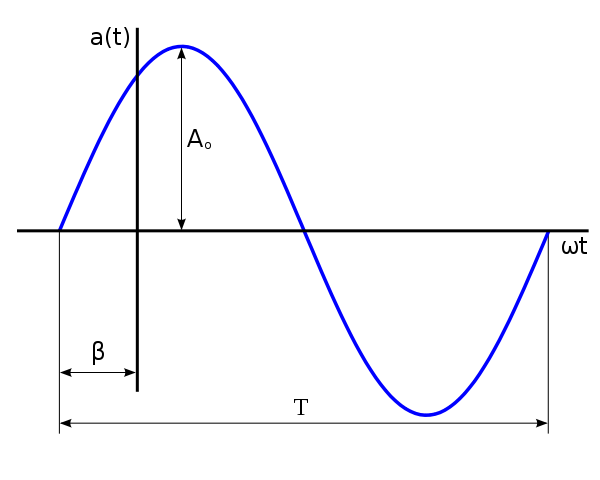
\includegraphics[scale=0.5]{Imagenes/600px-OndaSenoidal.png}
    \caption{Parámetros característicos de una oscilación sinusoidal.}
    \label{fig:ondaSenoidal}
\end{figure}

\section{Generador de funciones}

Un generador de funciones es un instrumento utilizado en la electrónica y sirve para generar o simular señales específicas con determinadas características. Por ejemplo, crear o simular una señal que puede ser cuadrada, sinusoidal, de una determinada frecuencia, y de una determinada amplitud. De esta forma, podemos aplicar esta señal generada a un circuito para ver su respuesta. Entonces, para resumir lo anterior, es un simulador de señales de diferentes características.\citep{GenFunc}



\section{Conceptos de tierra y masa}

\subsection{Tierra física}

El término "tierra física", como su nombre indica, se refiere al potencial de la superficie de la Tierra.\citep{TT}\\

 Para hacer la conexión de este potencial de tierra a un circuito eléctrico se usa un electrodo de tierra, que puede ser algo tan simple como una barra metálica (usualmente de cobre) anclada al suelo, a veces humedecida para una mejor conducción.\citep{TT}\\

Por último hay que decir que el potencial de la tierra no siempre se puede considerar constante, especialmente en el caso de caída de rayos. Por ejemplo si cae un rayo, a una distancia de 1 kilómetro del lugar en que cae, la diferencia de potencial entre dos puntos separados por 10 metros será de más de 150 V en ese instante.\citep{TT}\\

\subsection{Tierra analógica}

La definición clásica de tierra (en inglés de Estados Unidos ground de donde viene la abreviación GND, earth en inglés de Reino Unido) es un punto que servirá como referencia de tensiones en un circuito (0 voltios). El problema de la anterior definición es que, en la práctica, esta tensión varía de un punto a otro, es decir, debido a la resistencia de los cables y a la corriente que pasa por ellos, habrá una diferencia de tensión entre un punto y otro cualquiera de un mismo cable.\citep{TT}\\

Una definición más útil es que masa es la referencia de un conductor que es usado como retorno común de las corrientes.\citep{TT}\\

\section{Tierra virtual}

En electrónica, un tierra virtual es un nodo de un circuito que se mantiene a un potencial de referencia constante, sin estar conectado directamente con el potencial de referencia. En algunos casos se considera el potencial de referencia de la superficie de la tierra, y al nodo de referencia se llama "tierra" o "tierra" como consecuencia de ello.\citep{TieV}\\

El concepto de tierra virtual SIDA análisis de circuito amplificador operacional y otros circuitos y proporciona efectos útiles circuito práctico que serían difíciles de lograr por otros medios.\citep{TieV}\\

En teoría de circuitos, un nodo puede tener cualquier valor de corriente o voltaje pero implementaciones físicas de un suelo virtual tendrá limitaciones de capacidad de manejo actual y un cero impedancia que pueden tener efectos secundarios prácticos.\citep{TieV}\\

\section{Fusibles}

En electricidad, se denomina fusible a un dispositivo constituido por un soporte adecuado y un filamento o lámina de un metal o aleación de bajo punto de fusión que se intercala en un punto determinado de una instalación eléctrica para que se funda (por efecto Joule) cuando la intensidad de corriente supere (por un cortocircuito o un exceso de carga) un determinado valor que pudiera hacer peligrar la integridad de los conductores de la instalación con el consiguiente riesgo de incendio o destrucción de otros elementos.\citep{Fus}

\section{Tiristor}

El tiristor es una familia de componentes electrónicos constituido por elementos semiconductores que utiliza realimentación interna para producir una conmutación. Los materiales de los que se compone son de tipo semiconductor, es decir, dependiendo de la temperatura a la que se encuentren pueden funcionar como aislantes o como conductores. Son dispositivos unidireccionales (SCR) o bidireccionales (Triac) o (DIAC). Se emplea generalmente para el control de potencia eléctrica.\citep{Tirs}\\

Para los SCR el dispositivo consta de un ánodo y un cátodo, donde las uniones son de tipo P-N-P-N entre los mismos. Por tanto se puede modelar como 2 transistores típicos P-N-P y N-P-N, por eso se dice también que el tiristor funciona con tensión realimentada. Se crean así 3 uniones (denominadas J1, J2, J3 respectivamente), el terminal de puerta está a la unión J2 (unión NP).\citep{Tirs}\\

Algunas fuentes definen como sinónimos al tiristor y al rectificador controlado de silicio (SCR); Aunque en realidad la forma correcta es clasificar al SCR como un tipo de tiristor, a la par que los dispositivos DIAC y TRIAC.\citep{Tirs}\\

Este elemento fue desarrollado por ingenieros de General Electric en los años 1960. Aunque un origen más remoto de este dispositivo lo encontramos en el SCR creado por William Shockley (premio Nobel de física en 1956) en 1950, el cual fue defendido y desarrollado en los laboratorios Bell en 1956. Gordon Hall lideró el desarrollo en Morgan Stanley para su posterior comercialización por parte de Frank W. "Bill" Gutzwiller, de General Electric.\citep{Tirs}\\




\begin{figure}[h!]
    \centering
    \begin{subfigure}[b]{0.3\textwidth}
        \includegraphics[width=\textwidth]{Imagenes/scr-c106m.jpg}
        \caption{SCR}
        \label{fig:scr}
    \end{subfigure}
    ~ %add desired spacing between images, e. g. ~, \quad, \qquad, \hfill etc. 
      %(or a blank line to force the subfigure onto a new line)
    \begin{subfigure}[b]{0.3\textwidth}
        \includegraphics[width=\textwidth]{Imagenes/diac.png}
        \caption{DIAC}
        \label{fig:diac}
    \end{subfigure}
    ~ %add desired spacing between images, e. g. ~, \quad, \qquad, \hfill etc. 
    %(or a blank line to force the subfigure onto a new line)
    \begin{subfigure}[b]{0.3\textwidth}
        \includegraphics[width=\textwidth]{Imagenes/triac-q4015l5.jpg}
        \caption{TRIAC}
        \label{fig:triac}
    \end{subfigure}
    \caption{Ejemplos Tiristor}\label{fig:animals}
\end{figure}



\section{Circuito a resolver}

\begin{figure}[h!]
    \centering
    \includegraphics{}
    \begin{circuitikz}
\draw

(-1,0)--(-1,-1)
(-1,-1) to[V,l=$28v$](-1,-2) 
 (-1,-2)--(-1,-3)
 
 (-1,-3)to[R,l=$R_5$](2,-3)
 
 (-1,0) to[R,l=$R_1$](2,0)
 
 
 (2,-3)to[R,l=$R_3$](2,0)
 
 (2,0)to[R,l=$R_2$](5,0)
 (2,-3)--(5,-3)
 
  (5,-3)to[R,l=$R_4$](5,0)
 
 
;

%\draw[thick,arrows=->]
%(2.5,0)--(2.5,-1)
%;
 
\end{circuitikz}
    \caption{Circuito a resolver}
   \label{fig:circuito}
\end{figure}

\subsection{Resultados}

Para resolver el circuito se hicieron equivalente los resistores de 5 y 10 $\Omegas$ para obtener el voltaje en esas ramas, así se pudo deducir la corriente en la rama del resistor de 50 $\Omega$ y el circuito equivalente, posterirmente se usaron las leyes de Kirchhoff para deducir los voltajes y las corrientes respectivamente.

\begin{table}[h!]
\centering

\begin{tabular}{|c|c|c|}
\hline
Componente & V {[}V{]} & I {[}A{]} \\ \hline
R1       &    &      \\ \hline
R2       &      &     \\ \hline
R3        &       &     \\ \hline
R4        &       &     \\ \hline
R5        &       &     \\ \hline
V fuente   & 18        &      \\ \hline
\end{tabular}
\caption{Tabla de Resultados}
\label{tabla-resultados}

\end{table}

%.\\[100cm]
\bibliographystyle{plain}
\bibliography{previo2.bib}


\end{document}